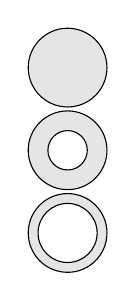
\begin{tikzpicture}[scale=0.5]
    \tikzset{
      reversed with radius/.style={
        x radius=#1,
        y radius=-#1,
     }
    }
    \draw[preaction={fill,opacity=0.1}] (0,0)
      circle[reversed with radius=1cm]
      circle[radius=0.75cm];
     %
     \draw[preaction={fill,opacity=0.1}] (0,2.1)
      circle[reversed with radius=1cm]
      circle[radius=0.5cm];
    %
    \draw[preaction={fill,opacity=0.1}] (0,4.2)
      circle[reversed with radius=1cm];
\end{tikzpicture}
%
%
%%%%%%%%%%%%%%%%%%%%%
% Sphere and Cylinder
%%%%%%%%%%%%%%%%%%%%%
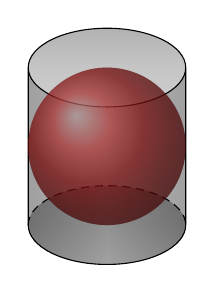
\begin{tikzpicture}
\def\R{1}
  \fill[top color    = gray!50!black,
        bottom color = gray!10,
        middle color = gray,
        shading      = axis,
        opacity      = 0.25]
    (0,0) circle (\R cm and 0.5cm);
  \fill[left color   = gray!50!black,
        right color  = gray!50!black,
        middle color = gray!50,
        shading      = axis,
        opacity      = 0.25]
    (\R,0) -- (\R,2*\R)  arc (360:180:\R cm and 0.5cm)
          -- (-\R,0) arc (180:360:\R cm and 0.5cm);
  \fill[top color    = gray!90!,
        bottom color = gray!2,
        middle color = gray!30,
        shading      = axis,
        opacity      = 0.25]
    (0,2*\R) circle (\R cm and 0.5cm);
  
  \draw (-\R,2*\R) -- (-\R,0) arc (180:360:\R cm and 0.5cm)
              -- (\R,2*\R) ++ (-\R,0) circle (\R cm and 0.5cm);
  \draw[densely dashed] (-\R,0) arc (180:0:\R cm and 0.5cm);
 \fill[thick, ball color=red!90, opacity = 0.5] (0,\R) circle (\R);
% \fill[thick, ball color=orange!90, opacity = 0.5] (0,3*\R) circle (\R);
% \fill[thick, ball color=blue!90, opacity = 0.5] (0,5*\R) circle (\R);
 \end{tikzpicture}